\chapter{Benchmarks}

In this chapter, we measure the performance of our implementation. We quantify the impact of different input size and algorithm parameters. In the end, we compare our implementation with an original python implementation of the algorithm.

All the data was measured using an NVIDIA RTX 3080 graphics card with Intel i5 6600K processor. We used an M.2 SSD disk.


\section{Relative performance of individual parts}

\begin{figure}
	\centering
	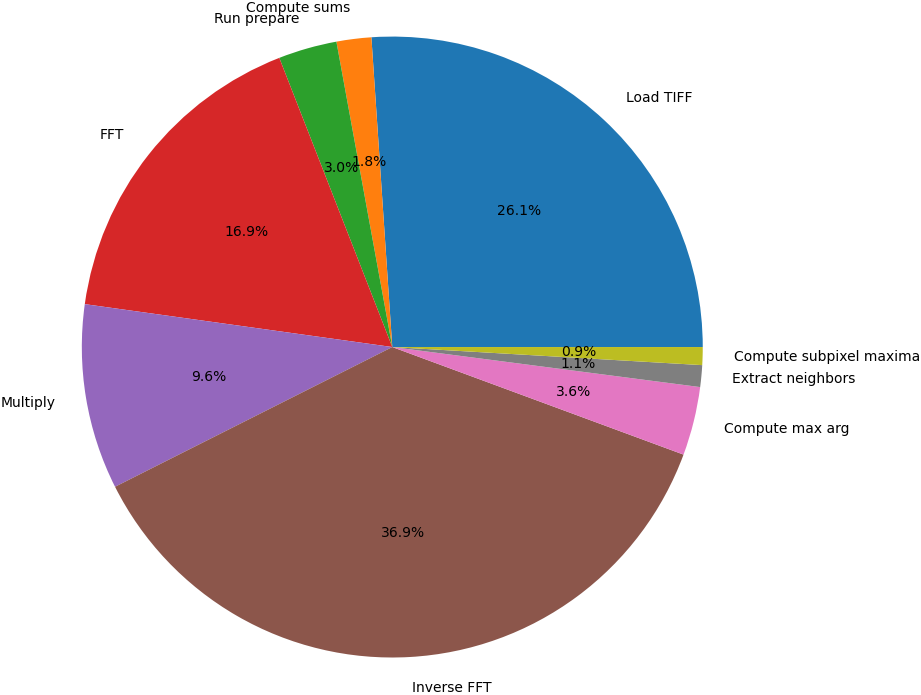
\includegraphics[width=\textwidth]{img/eval/individual-parts}
	\caption{Relative performance of individual parts of the algorithm. The data was measured from a run of the algorithm with a configuration of 90 subregions with size $100 \times 100$.}
	\label{individual-parts}
\end{figure}

We begin with an overview of all the kernels used in the implementation. \Cref{individual-parts} shows how much time the implementation spends in individual kernels. We can see, that the most demanding parts are loading of the TIFF and the cross--correlation, which is computed using the multiply kernel and the Fourier transforms. 

\section{Cross--correlation}
First, we measure the difference between the cross--correlation algorithms.

(Do jedneho grafu vsetky velkosti )


\section{Float versus double}




\section{Speedup compared to original python implementation}

overall performance - compare with python

batch size for different subregion sizes and count

different subregion sizes and count

sum - compare N to size of one slice, to batch size, to number of slices - how?